\chapter{Introdução}

\section{Contexto}

Medir a qualidade do código-fonte  de um software é um processo fundamental no seu desenvolvimento, pois daí surgem indicadores sobre os efeitos que uma alteração no código irá causar ou sobre os efeitos gerados na qualidade do software após a adesão de uma nova prática na equipe de desenvolvimento \cite{Fenton98}. 

Através do processo de medição da qualidade interna do software é possível não só entender e controlar o que está se passando no seu desenvolvimento, como também ser encorajado a tomar decisões que visem a sua melhoria \cite{Fenton98}. Como a qualidade do código fonte está relacionada à qualidade interna do produto de software \cite{ISO25023}, sua medição, e consequentemente as melhorias implantadas nele melhoram a qualidade do produto como um todo. 
 

\section{Justificativa}

Buscando facilitar a interpretação das métricas de código fonte, bem como apoiar as decisões de refatoração a serem tomadas, \citeonline{rego_monitoramento_2014} elaborou um ambiente de \textit{Data Warehouse} para armazenamento de métricas, sobre o qual esse trabalho irá analisar sua eficácia e eficiência no monitoramento da qualidade interna do software, sendo essa sua maior contribuição. Essa análise poderá ajudar equipes de desenvolvimento de software na escolha de uma maneira de aferir a qualidade interna do seu produto e tomar as decisões corretas sobre o que refatorar.

\section{Problema}

ESCREVER PROBLEMA

Baseando-se no problema descrito, foi criada a seguinte questão geral de pesquisa:

\textbf{\textit{O uso de \textit{Data Warehousing} é eficaz e eficiente no monitoramento de métricas de código fonte, facilitando a interpretação dos resultados da análise estática e apoiando decisões de refatoração?} }

\section{Objetivos}

O objetivo geral desse trabalho consiste na análise da eficácia e eficiência do uso de \textit{Data Warehousing} no monitoramento de métricas de código fonte. Como esse trabalho é dividido em duas partes, seus objetivos também foram divididos dessa forma, sendo os objetivos da primeira parte:

\begin{easylist}[itemize]	
	
	& Levantar fundamentação teórica que servirá de base para todo o trabalho.
	& Apresentar solução desenvolvida por \citeonline{rego_monitoramento_2014} para monitoramento de métricas através de \textit{Data Warehousing}. 
	& Elaborar o projeto do estudo de caso.
	
	\end{easylist}	

A segunda parte desse trabalho, a ser desenvolvida no primeiro semestre de 2015, terá os seguintes objetivos:	

\begin{easylist}[itemize]	
	
	& Coletar os dados que surgirão como respostas das questões específicas elaboradas para o estudo de caso, como por exemplo o nível de satisfação quanto ao uso da solução ou qual a taxa de oportunidade de melhoria de código em um determinado intervalo de tempo.
	& Realizar análise dos dados coletados.
	& Relatar resultados obtidos.
	
	\end{easylist}

\section{Metodologia de pesquisa}

A metodologia adotada:

Segundo \citeonline{wohlin2012experimentation} a condução de um estudo de caso deve obedecer os cinco passos listados de forma sequencial na figura \ref{fig:estudodecaso}: 

\begin{figure}[h!]
\centering
\includegraphics[keepaspectratio=false,scale=0.8]{figuras/figuras_matheus/estudodecaso.eps}
\caption{Estrutura do estudo de caso}
\label{fig:estudodecaso}
\end{figure}
\FloatBarrier

Projetar o estudo de caso e preparar a coleta de dados são etapas que consistem em uma macro atividade chamada de planejamento do estudo de caso. Nesse planejamento serão identificados elementos como o problema a ser resolvido e a questão de pesquisa a ser respondida, de modo que o protocolo de estudo de caso possa ser elaborado já determinando qual o método e a fonte da coleta dos dados. Coletar dados é uma atividade a ser executada em seguida, feita através de pesquisas bibliográficas e documentais além dos resultados extraídos da própria solução para monitoramento de código fonte a ser analisada durante o estudo de caso. Analisar os dados coletados diz respeito à interpretação dos dados coletados compreendendo não só análises quantitativas como também qualitativas. A etapa chamada de compartilhar os resultados, por sua vez, indica que os resultados coletados e interpretados são expostos nesse trabalho a quem desejar fazer sua leitura. 


\section{Organização do Trabalho}

Esse trabalho está dividido em 5 capítulos:

	\begin{easylist}[itemize]	
	
	& \textbf{Capítulo 1 - Introdução:} Esse capítulo tem como objetivo apresentar o contexto que esse trabalho está inserido, o problema sobre o qual ele buscará resolver, qual a justificativa e os objetivos da sua realização e como essa pequisa foi elaborada.
	& \textbf{Capítulo 2 - Métricas de Software:} Capítulo responsável pela explicação teórica a respeito do que são métricas de código e como elas foram utilizadas no desenvolvimento da solução que esse trabalho busca analisar.
	& \textbf{Capítulo 3 - Data Warehouse:} Nesse capítulo serão apresentados conceitos teóricos sobre \textit{Data Warehousing}, assim como a maneira como foi desenvolvido o ambiente de \textit{Data Warehouse} para armazenamento de métricas de código fonte.
	& \textbf{Capítulo 4 - Projeto de estudo de caso:} Será apresentada a estratégia de pesquisa adotada durante o trabalho, buscando elaborar um protocolo para o estudo de caso que será realizado. Elementos de pesquisa como o problema a ser resolvido, os objetivos a serem alcançados no estudo de caso e quais os métodos de coleta e análise dos dados serão identificados e explicados.
	& \textbf{Capítulo 5 - Conclusão:} Além das considerações finais dessa primeira parte do trabalho, serão descritos objetivos para a segunda parte a ser realizada ao término desta.
	
	\end{easylist}	
